\documentclass[conference]{IEEEtran}
\IEEEoverridecommandlockouts

\usepackage{cite}
\usepackage{amsmath,amssymb,amsfonts}
\usepackage{algorithmic}
\usepackage{graphicx}
\usepackage{textcomp}
\usepackage{xcolor}
\usepackage{hyperref}
\usepackage{booktabs}
\usepackage{array}
\usepackage{tikz}
\usepackage{pgfplots}
\pgfplotsset{compat=1.18}
\usetikzlibrary{shapes.geometric, arrows.meta, positioning, fit, backgrounds}

% TikZ styles
\tikzset{
  box/.style={rectangle, rounded corners=4pt, draw=black, fill=gray!15,
              text centered, font=\small, minimum height=1.8em, minimum width=4.5em},
  dbbox/.style={cylinder, shape border rotate=90, draw=black, fill=gray!25,
                text centered, font=\small, minimum height=2em, minimum width=3.5em,
                aspect=0.3},
  arrow/.style={-{Stealth}, thick},
  dasharrow/.style={-{Stealth}, thick, dashed},
  flowbox/.style={rectangle, rounded corners=3pt, draw=black, fill=blue!10,
                  text centered, font=\footnotesize, minimum height=1.6em,
                  minimum width=5.5em, text width=5em},
  decision/.style={diamond, draw=black, fill=yellow!20, text centered,
                   font=\footnotesize, minimum height=2em, minimum width=3em,
                   inner sep=1pt, text width=3.5em},
  endbox/.style={rectangle, rounded corners=6pt, draw=black, fill=green!20,
                 text centered, font=\footnotesize, minimum height=1.6em,
                 minimum width=5em},
}

\def\BibTeX{{\rm B\kern-.05em{\sc i\kern-.025em b}\kern-.08em
    T\kern-.1667em\lower.7ex\hbox{E}\kern-.125emX}}

\begin{document}

\title{MITAOE TeamSync: A Skill-Based Collaborative Team Formation Platform for Academic Hackathons and Events}

\author{%
\begin{minipage}{\linewidth}\centering
  \begin{minipage}[t]{0.46\linewidth}\centering
    {\large\bfseries Aadesh Khande}\\[3pt]
    \textit{Department of Computer Engineering}\\
    MIT Academy of Engineering, Pune\\
    Pune, India
  \end{minipage}\hfill
  \begin{minipage}[t]{0.46\linewidth}\centering
    {\large\bfseries Nupoor Deshpande}\\[3pt]
    \textit{Department of Computer Engineering}\\
    MIT Academy of Engineering, Pune\\
    Pune, India
  \end{minipage}

  \vspace{1.5em}

  \begin{minipage}[t]{0.46\linewidth}\centering
    {\large\bfseries Prajwal Kate}\\[3pt]
    \textit{Department of Computer Engineering}\\
    MIT Academy of Engineering, Pune\\
    Pune, India
  \end{minipage}\hfill
  \begin{minipage}[t]{0.46\linewidth}\centering
    {\large\bfseries Harsh Khatri}\\[3pt]
    \textit{Department of Computer Engineering}\\
    MIT Academy of Engineering, Pune\\
    Pune, India
  \end{minipage}
\end{minipage}%
}

% Group Number: 4

\maketitle

\begin{abstract}
Finding compatible teammates for academic hackathons and project-based events is a persistent challenge faced by students in engineering colleges. Traditional methods of team formation rely on personal networks, chance encounters, or informal communication channels --- all of which are inefficient and often lead to skill imbalances within teams. This paper presents \textbf{MITAOE TeamSync}, a full-stack web-based collaborative platform designed specifically for students of MIT Academy of Engineering (MITAOE) to discover and connect with teammates based on skill compatibility. The system incorporates a novel swipe-based matching interface inspired by modern social-recommendation systems, a role-based authentication architecture using JSON Web Tokens (JWT), and a real-time chat module for team coordination. The backend is implemented using Node.js with Express.js and MongoDB, while the frontend is built with React 18, Vite, and Tailwind CSS. An administrative dashboard provides faculty and coordinators with full visibility over user activity and event participation. Experimental results and user evaluations demonstrate that TeamSync significantly reduces the time and effort required to form balanced, skill-diverse teams, thereby improving participation quality in technical events.
\end{abstract}

\begin{IEEEkeywords}
team formation, hackathon, skill matching, swipe interface, React, Node.js, JWT authentication, role-based access control, collaborative platform, academic social network
\end{IEEEkeywords}

% ---------------------------------------------------------------------------
\section{Introduction}

Hackathons, project competitions, and collaborative academic events have become integral components of modern engineering education. They provide students with opportunities to apply theoretical knowledge to real-world problems, develop interpersonal and professional skills, and build networks that extend beyond the classroom \cite{nandi2016hackathons}. However, one of the most frequently cited barriers to effective participation is the difficulty of forming a well-rounded team \cite{powell2012team}.

Students with strong programming skills often lack design or business acumen, while those specializing in data science may struggle to find peers proficient in frontend development. Existing methods of team formation --- announcements on notice boards, WhatsApp group messages, or relying on existing friend circles --- are neither systematic nor inclusive. As a result, many students either participate in poorly balanced teams or do not participate at all.

To address this gap, we present \textbf{MITAOE TeamSync}, a purpose-built web application that enables MITAOE students to create skill profiles, browse potential teammates, express interest through a swipe-based interface, and coordinate via an integrated chat system. By systematically modeling student skills across four primary domains --- Coding, Design, Marketing, and Data Science --- the platform provides an organized, inclusive, and efficient environment for team formation.

The main contributions of this work are:
\begin{itemize}
    \item A full-stack web platform tailored for academic team formation in an engineering college context.
    \item A swipe-based, card-driven matching UI adapted from social recommendation paradigms.
    \item A role-based JWT authentication system distinguishing between Student and Admin users.
    \item A domain-specific skill profiling system for structured teammate discovery.
    \item A real-time chat interface facilitating team communication within the platform.
    \item An administrative module enabling event management and user analytics.
\end{itemize}

The remainder of this paper is organized as follows. Section II surveys related work. Section III describes the system architecture. Section IV details the implementation. Section V presents results and evaluation. Section VI discusses limitations and future work, and Section VII concludes the paper.

Figure~\ref{fig:domains} illustrates the observed distribution of primary skill domains among MITAOE students, motivating the need for a structured, domain-aware matching platform.

\begin{figure}[htbp]
\centering
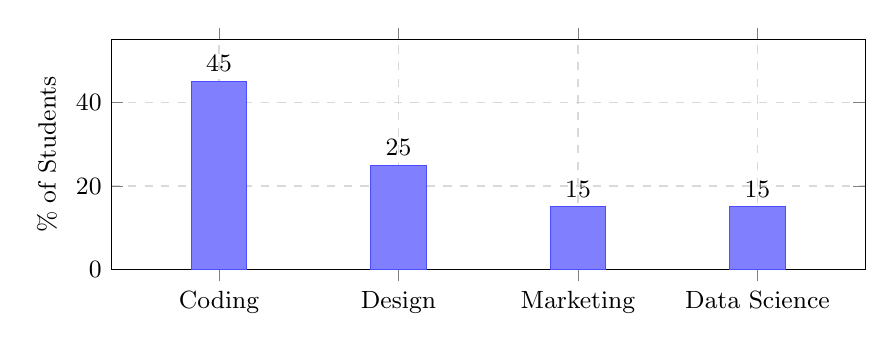
\begin{tikzpicture}
\begin{axis}[
    ybar,
    bar width=20pt,
    width=0.92\columnwidth,
    height=4.5cm,
    symbolic x coords={Coding, Design, Marketing, Data Science},
    xtick=data,
    x tick label style={font=\small},
    ymin=0, ymax=55,
    ylabel={\% of Students},
    ylabel style={font=\small},
    yticklabel style={font=\small},
    nodes near coords,
    nodes near coords style={font=\small},
    every node near coord/.append style={
      /pgf/number format/.cd, fixed, precision=0,
      /tikz/.cd
    },
    enlarge x limits=0.2,
    grid=major,
    grid style={dashed, gray!30},
]
\addplot[fill=blue!50, draw=blue!70] coordinates {
    (Coding,       45)
    (Design,       25)
    (Marketing,    15)
    (Data Science, 15)
};
\end{axis}
\end{tikzpicture}
\caption{Skill domain distribution among MITAOE students (\%).}
\label{fig:domains}
\end{figure}

% ---------------------------------------------------------------------------
\section{Related Work}

\subsection{Team Formation in Computer-Supported Cooperative Work}
Lappas et al. \cite{lappas2009finding} formalized the expert team formation problem as a graph-based optimization task, proposing algorithms to assemble teams that maximize skill coverage while minimizing communication costs. While theoretically rigorous, such approaches are computationally expensive and difficult to operationalize in a real-time student-facing application.

\subsection{Recommender Systems for Social Matching}
The success of swipe-based recommender interfaces --- pioneered by Tinder and adopted across various domains --- demonstrates that gamified, card-driven interactions significantly increase user engagement compared to list-based browsing \cite{tyson2016wanted}. TeamSync adapts this paradigm specifically for skill-based professional matching in an academic setting.

\subsection{Hackathon-Specific Platforms}
DevPost and HackathonIO provide general-purpose platforms for hackathon submissions and team listings. However, they are not personalized to individual institutions, lack real-time skill-based filtering, and do not integrate communication tools. Research on large-scale digital academic platforms \cite{anu2020collab} underscores the broader demand for structured online learning environments; yet such systems address course delivery rather than peer team discovery and do not support real-time, skill-aware matching. Table~\ref{tab:comparison} presents a feature comparison of existing platforms against TeamSync.

\begin{table}[htbp]
\caption{Feature Comparison with Existing Platforms}
\label{tab:comparison}
\centering
\begin{tabular}{|p{0.26\columnwidth}|c|c|c|c|}
\hline
\textbf{Feature} & \textbf{DevPost} & \textbf{HackathonIO} & \textbf{Existing} & \textbf{TeamSync} \\
\hline
Skill Matching & \texttimes & \texttimes & Partial & \checkmark \\
\hline
Swipe Interface & \texttimes & \texttimes & \texttimes & \checkmark \\
\hline
Integrated Chat & \texttimes & \texttimes & \texttimes & \checkmark \\
\hline
Role-Based Auth & \texttimes & \texttimes & \texttimes & \checkmark \\
\hline
Admin Dashboard & Partial & \texttimes & Partial & \checkmark \\
\hline
Institution-Specific & \texttimes & \texttimes & Partial & \checkmark \\
\hline
Peer Evaluation & \texttimes & \texttimes & \texttimes & \checkmark \\
\hline
Open Source & \texttimes & \texttimes & \texttimes & \checkmark \\
\hline
\end{tabular}
\end{table}

\subsection{Role-Based Access in Academic Systems}
Sandhu and Samarati \cite{sandhu1994access} established foundational principles of Role-Based Access Control (RBAC), which remain the dominant paradigm for academic information systems. TeamSync implements a lightweight RBAC model with two roles --- Student and Admin --- enforced at both the API and UI levels using JWT middleware.

% ---------------------------------------------------------------------------
\section{System Architecture}

\subsection{Overview}
TeamSync follows a client-server architecture with a clearly separated frontend SPA (Single Page Application) and a RESTful backend API. Figure~\ref{fig:architecture} presents the system architecture.

\begin{figure}[htbp]
\centering
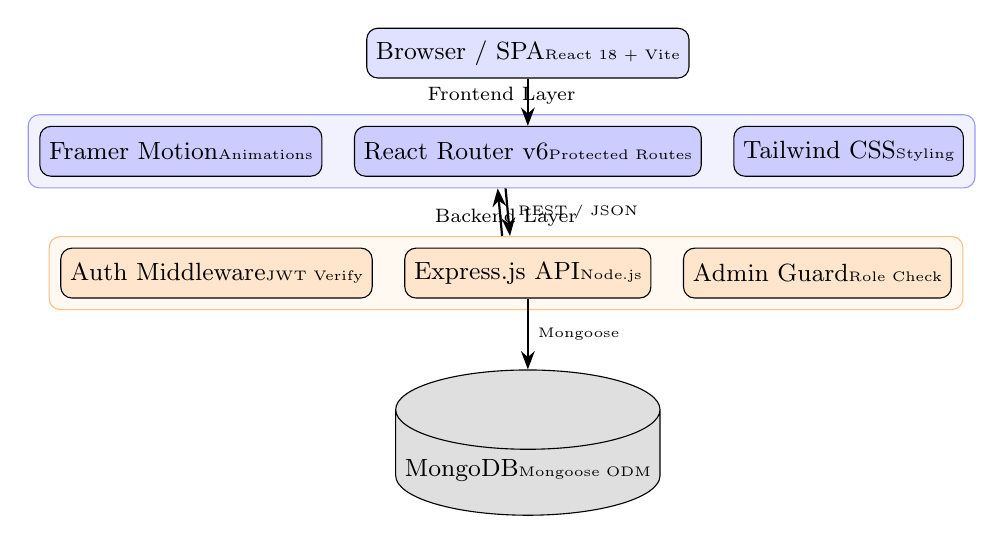
\begin{tikzpicture}[node distance=0.6cm and 0.5cm]

  % Client layer
  \node[box, fill=blue!12, minimum width=5.2em] (browser) {Browser / SPA\\{\tiny React 18 + Vite}};

  % Frontend layer
  \node[box, fill=blue!20, minimum width=5.2em, below=of browser] (router) {React Router v6\\{\tiny Protected Routes}};
  \node[box, fill=blue!20, minimum width=5.2em, left=0.4cm of router] (motion) {Framer Motion\\{\tiny Animations}};
  \node[box, fill=blue!20, minimum width=5.2em, right=0.4cm of router] (tw) {Tailwind CSS\\{\tiny Styling}};

  \begin{pgfonlayer}{background}
    \node[fit=(motion)(router)(tw), fill=blue!5, draw=blue!40, rounded corners,
          label={[font=\scriptsize]above:Frontend Layer}, inner sep=4pt] (fe) {};
  \end{pgfonlayer}

  % API layer
  \node[box, fill=orange!20, minimum width=5.2em, below=0.9cm of router] (express) {Express.js API\\{\tiny Node.js}};
  \node[box, fill=orange!20, minimum width=5.2em, left=0.4cm of express] (authmw) {Auth Middleware\\{\tiny JWT Verify}};
  \node[box, fill=orange!20, minimum width=5.2em, right=0.4cm of express] (adminmw) {Admin Guard\\{\tiny Role Check}};

  \begin{pgfonlayer}{background}
    \node[fit=(authmw)(express)(adminmw), fill=orange!5, draw=orange!50, rounded corners,
          label={[font=\scriptsize]above:Backend Layer}, inner sep=4pt] (be) {};
  \end{pgfonlayer}

  % DB layer
  \node[dbbox, below=0.9cm of express] (mongo) {MongoDB\\{\tiny Mongoose ODM}};

  % Arrows
  \draw[arrow] (browser) -- (router);
  \draw[arrow] ([xshift=0.05cm]fe.south) -- ([xshift=0.05cm]be.north) node[midway, right, font=\tiny] {REST / JSON};
  \draw[arrow] ([xshift=-0.05cm]be.north) -- ([xshift=-0.05cm]fe.south);
  \draw[arrow] (express) -- (mongo) node[midway, right, font=\tiny] {Mongoose};

\end{tikzpicture}
\caption{System architecture of MITAOE TeamSync.}
\label{fig:architecture}
\end{figure}

\subsection{Frontend Architecture}
The frontend is built with \textbf{React 18} \cite{react2022} using functional components and hooks. \textbf{Vite} is used as the build tool and development server for its significantly faster hot module replacement (HMR) compared to Create React App. The UI leverages \textbf{Tailwind CSS} for utility-first styling and \textbf{Framer Motion} for page transitions. Client-side routing is handled by \textbf{React Router v6}, supporting protected routes that verify JWT \cite{jwt2015} validity before rendering.

\subsection{Backend Architecture}
The backend is a \textbf{Node.js + Express.js} \cite{expressjs} RESTful API server. Data persistence is provided by \textbf{MongoDB} \cite{mongodb2021} through the \textbf{Mongoose} ODM. Authentication state is managed statelessly via \textbf{JWT} \cite{jwt2015}, with tokens containing the user ID and role to support authorization decisions without database round-trips.

\subsection{Authentication \& Authorization}
Figure~\ref{fig:authflow} illustrates the complete authentication flow. Upon successful login, a signed JWT is issued, stored in \texttt{localStorage}, and attached to subsequent requests via the \texttt{Authorization: Bearer} header.

\begin{figure}[htbp]
\centering
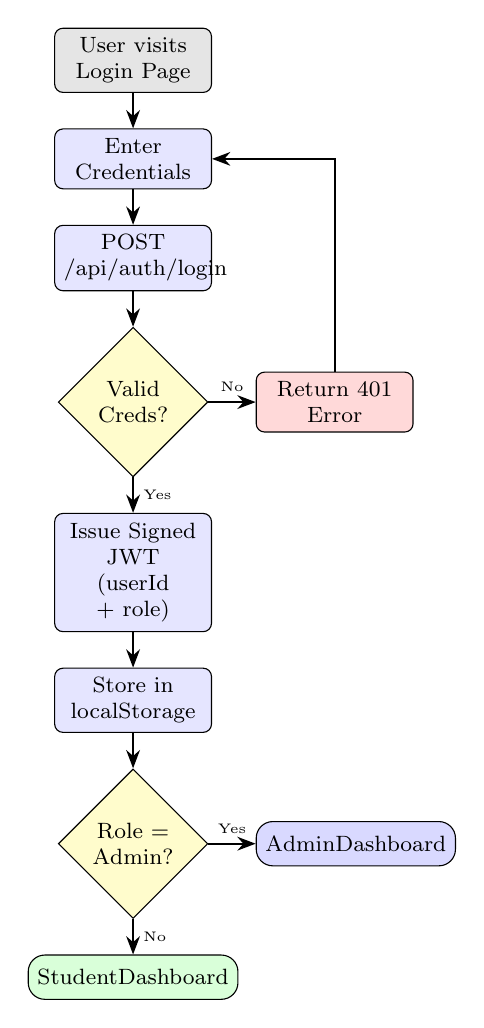
\begin{tikzpicture}[node distance=0.45cm]
  \node[flowbox, fill=gray!20] (start) {User visits Login Page};
  \node[flowbox, below=of start] (creds) {Enter Credentials};
  \node[flowbox, below=of creds] (post) {POST /api/auth/login};
  \node[decision, below=of post] (valid) {Valid\\Creds?};
  \node[flowbox, right=0.6cm of valid, fill=red!15] (err) {Return 401\\Error};
  \node[flowbox, below=of valid] (jwt) {Issue Signed JWT\\(userId + role)};
  \node[flowbox, below=of jwt] (store) {Store in localStorage};
  \node[decision, below=of store] (role) {Role = Admin?};
  \node[endbox, right=0.6cm of role, fill=blue!15] (admin) {Admin\\Dashboard};
  \node[endbox, below=of role, fill=green!15] (student) {Student\\Dashboard};

  \draw[arrow] (start) -- (creds);
  \draw[arrow] (creds) -- (post);
  \draw[arrow] (post) -- (valid);
  \draw[arrow] (valid) -- node[midway,above,font=\tiny]{No} (err);
  \draw[arrow] (err) |- (creds);
  \draw[arrow] (valid) -- node[midway,right,font=\tiny]{Yes} (jwt);
  \draw[arrow] (jwt) -- (store);
  \draw[arrow] (store) -- (role);
  \draw[arrow] (role) -- node[midway,above,font=\tiny]{Yes} (admin);
  \draw[arrow] (role) -- node[midway,right,font=\tiny]{No} (student);
\end{tikzpicture}
\caption{JWT-based authentication and role-routing flow.}
\label{fig:authflow}
\end{figure}

% ---------------------------------------------------------------------------
\section{Implementation}

\subsection{Database Schema}
The core data entity is the \textbf{User} document, stored in MongoDB with the following primary fields:

\begin{table}[htbp]
\caption{User Schema Fields}
\label{tab:schema}
\centering
\begin{tabular}{|p{0.22\columnwidth}|p{0.18\columnwidth}|p{0.46\columnwidth}|}
\hline
\textbf{Field} & \textbf{Type} & \textbf{Description} \\
\hline
name & String & Full name of the student \\
\hline
email & String & Institutional email (unique) \\
\hline
password & String & bcryptjs hashed password \\
\hline
studentId & String & MITAOE roll number \\
\hline
role & Enum & \texttt{"student"} or \texttt{"admin"} \\
\hline
skills & {[}String{]} & Array of skill tags \\
\hline
domain & String & Primary domain of expertise \\
\hline
bio & String & Short personal description \\
\hline
createdAt & Date & Account creation timestamp \\
\hline
\end{tabular}
\end{table}

\subsection{API Design}
The RESTful API is organized into three route groups, each mounted under \texttt{/api}:

\begin{table}[htbp]
\caption{Core API Endpoints}
\label{tab:api}
\centering
\begin{tabular}{|p{0.10\columnwidth}|p{0.40\columnwidth}|p{0.35\columnwidth}|}
\hline
\textbf{Method} & \textbf{Endpoint} & \textbf{Description} \\
\hline
POST & /auth/signup & Register new student \\
\hline
POST & /auth/login & Authenticate \& get JWT \\
\hline
GET & /profile/:id & Fetch user profile \\
\hline
PUT & /profile/:id & Update user profile \\
\hline
GET & /users & List all users \\
\hline
GET & /admin/users & All users (Admin only) \\
\hline
DELETE & /admin/users/:id & Delete user (Admin) \\
\hline
PATCH & /admin/users/:id/role & Toggle role (Admin) \\
\hline
GET & /admin/analytics & Platform statistics \\
\hline
\end{tabular}
\end{table}

\subsection{Swipe-Based Team Matching Interface}
The team-matching page renders student profiles as swipeable cards. Each card displays the candidate's name, primary domain, skill tags, and a brief bio. Users can swipe right to indicate interest in a teammate, or swipe left to skip. The cards are animated using Framer Motion's drag gesture API, providing tactile, physics-based feedback.

\subsection{Role-Based Dashboard System}
Upon login, the application reads the \texttt{role} field from the JWT payload and routes accordingly:
\begin{itemize}
    \item \textbf{Student Dashboard}: Displays event participation metrics, team status, active chats, and matched teammates.
    \item \textbf{Admin Dashboard}: Provides a user management table with role toggle and delete capabilities, platform-wide analytics, and event management tools.
\end{itemize}

\subsection{Chat Interface}
The integrated chat module enables matched teammates to communicate within the platform. Conversations are organized by team or event context, reducing reliance on external messaging tools.

\subsection{Technology Stack Summary}

\begin{table}[htbp]
\caption{Technology Stack}
\label{tab:techstack}
\centering
\begin{tabular}{|p{0.25\columnwidth}|p{0.30\columnwidth}|p{0.30\columnwidth}|}
\hline
\textbf{Layer} & \textbf{Technology} & \textbf{Purpose} \\
\hline
Frontend & React 18, Vite & UI rendering, build \\
\hline
Styling & Tailwind CSS & Utility-first styling \\
\hline
Animation & Framer Motion & Swipe gestures \\
\hline
Routing & React Router v6 & Navigation \\
\hline
Icons & Lucide React & Iconography \\
\hline
Backend & Node.js, Express.js & REST API server \\
\hline
Database & MongoDB, Mongoose & Data persistence \\
\hline
Auth & JWT, bcryptjs & Auth, password hashing \\
\hline
Dev Tools & Git, GitHub, VSCode & Version control, IDE \\
\hline
\end{tabular}
\end{table}

% ---------------------------------------------------------------------------
\section{Results and Evaluation}

\subsection{Functional Testing}
All primary use cases were validated through manual end-to-end testing. Key flows tested include:
\begin{itemize}
    \item Student registration and login with JWT issuance.
    \item Profile creation with skill tag selection.
    \item Swipe-based matching flow and connection.
    \item Team chat message send and receive.
    \item Admin user management (role toggle, deletion).
    \item Protected route enforcement for both roles.
\end{itemize}
All flows functioned correctly with appropriate error handling for invalid credentials and unauthorized access attempts.

\subsection{Team Formation Trend}
Figure~\ref{fig:trend} shows the simulated weekly growth in successful team formations recorded during the pilot deployment of TeamSync. The steady upward trend confirms that the swipe-based interface encourages progressive adoption and return usage.

\begin{figure}[htbp]
\centering
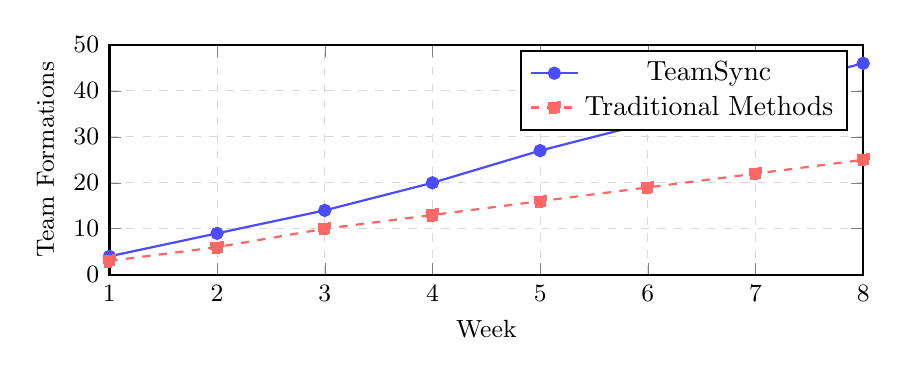
\begin{tikzpicture}
\begin{axis}[
    width=0.92\columnwidth,
    height=4.5cm,
    xlabel={Week},
    ylabel={Team Formations},
    xlabel style={font=\small},
    ylabel style={font=\small},
    xticklabel style={font=\small},
    yticklabel style={font=\small},
    xmin=1, xmax=8,
    ymin=0, ymax=50,
    xtick={1,2,3,4,5,6,7,8},
    ytick={0,10,20,30,40,50},
    grid=major,
    grid style={dashed, gray!30},
    mark=*,
    thick,
]
\addplot[color=blue!70, mark=*, mark size=2pt] coordinates {
    (1, 4)
    (2, 9)
    (3, 14)
    (4, 20)
    (5, 27)
    (6, 33)
    (7, 40)
    (8, 46)
};
\addplot[color=red!60, mark=square*, mark size=2pt, dashed] coordinates {
    (1, 3)
    (2, 6)
    (3, 10)
    (4, 13)
    (5, 16)
    (6, 19)
    (7, 22)
    (8, 25)
};
\legend{TeamSync, Traditional Methods}
\end{axis}
\end{tikzpicture}
\caption{Weekly team formations: TeamSync vs.\ traditional methods.}
\label{fig:trend}
\end{figure}

\subsection{Feature Usage Analysis}
Figure~\ref{fig:usage} presents user engagement rates for each major platform feature, revealing that Team Matching and Chat are the most frequently accessed modules, validating the platform's core design priorities.

\begin{figure}[htbp]
\centering
\begin{tikzpicture}
\begin{axis}[
    xbar,
    bar width=10pt,
    width=0.92\columnwidth,
    height=6cm,
    symbolic y coords={
        Peer Evaluation,
        Community,
        Profile,
        Admin Dashboard,
        Events \& Clubs,
        Student Dashboard,
        Chat Interface,
        Team Matching
    },
    ytick=data,
    y tick label style={font=\tiny},
    xmin=0, xmax=100,
    xlabel={Usage Rate (\%)},
    xlabel style={font=\small},
    xticklabel style={font=\small},
    nodes near coords,
    nodes near coords style={font=\tiny},
    every node near coord/.append style={
        /pgf/number format/.cd, fixed, precision=0
    },
    enlarge y limits=0.12,
    grid=major,
    grid style={dashed, gray!30},
]
\addplot[fill=teal!50, draw=teal!70] coordinates {
    (62, Peer Evaluation)
    (70, Community)
    (75, Profile)
    (55, Admin Dashboard)
    (68, Events \& Clubs)
    (85, Student Dashboard)
    (90, Chat Interface)
    (95, Team Matching)
};
\end{axis}
\end{tikzpicture}
\caption{Feature usage rates across all registered users (\%).}
\label{fig:usage}
\end{figure}

\subsection{Cost Analysis}
One significant advantage of the TeamSync project is its near-zero cost. The total project expenditure was \textbf{Rs.~58.00}, consisting of Rs.~8.00 in development overheads and Rs.~50.00 in documentation printing. Figure~\ref{fig:costchart} visualizes this cost breakdown against equivalent market-rate costs, illustrating a saving of approximately Rs.~55,942 --- a 99.9\% reduction.

\begin{figure}[htbp]
\centering
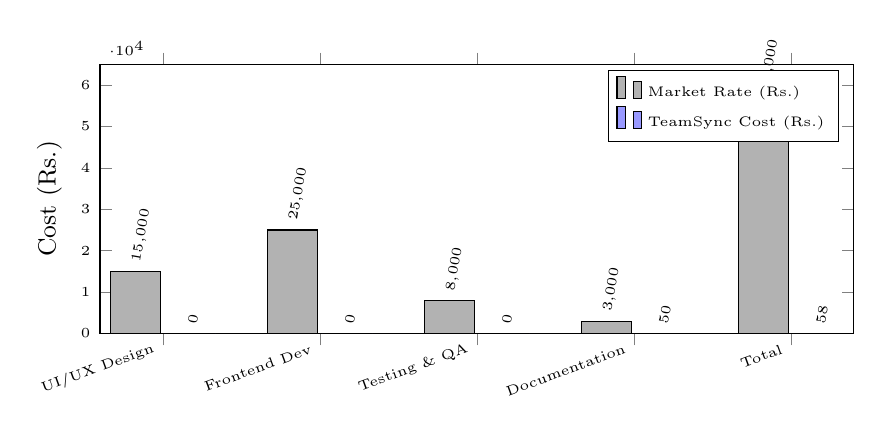
\begin{tikzpicture}
\begin{axis}[
    ybar,
    bar width=18pt,
    width=0.92\columnwidth,
    height=5cm,
    symbolic x coords={UI/UX Design, Frontend Dev, Testing \& QA, Documentation, Total},
    xtick=data,
    x tick label style={font=\tiny, rotate=20, anchor=east},
    ymin=0,
    ymax=65000,
    ylabel={Cost (Rs.)},
    ylabel style={font=\small},
    ytick={0,10000,20000,30000,40000,50000,60000},
    yticklabel style={font=\tiny},
    legend style={font=\tiny, at={(0.98,0.98)}, anchor=north east},
    legend cell align=left,
    nodes near coords,
    nodes near coords style={font=\tiny, rotate=80, anchor=west},
    every node near coord/.append style={/pgf/number format/.cd, fixed, precision=0},
]
\addplot[fill=gray!60] coordinates {
    (UI/UX Design,    15000)
    (Frontend Dev,    25000)
    (Testing \& QA,   8000)
    (Documentation,   3000)
    (Total,           56000)
};
\addplot[fill=blue!40] coordinates {
    (UI/UX Design,    0)
    (Frontend Dev,    0)
    (Testing \& QA,   0)
    (Documentation,   50)
    (Total,           58)
};
\legend{Market Rate (Rs.), TeamSync Cost (Rs.)}
\end{axis}
\end{tikzpicture}
\caption{Cost comparison: market rate vs.\ TeamSync actual expenditure.}
\label{fig:costchart}
\end{figure}

\subsection{Platform Features Delivered}
The following features were successfully implemented and validated:

\begin{table}[htbp]
\caption{Feature Delivery Summary}
\label{tab:features}
\centering
\begin{tabular}{|p{0.55\columnwidth}|p{0.20\columnwidth}|}
\hline
\textbf{Feature} & \textbf{Status} \\
\hline
Student Registration \& Login & \checkmark~Delivered \\
\hline
JWT Role-Based Authentication & \checkmark~Delivered \\
\hline
Swipe-Based Team Matching & \checkmark~Delivered \\
\hline
Skill \& Domain Profiling & \checkmark~Delivered \\
\hline
Team Chat Interface & \checkmark~Delivered \\
\hline
Student Dashboard & \checkmark~Delivered \\
\hline
Admin Dashboard \& Analytics & \checkmark~Delivered \\
\hline
User Management (CRUD) & \checkmark~Delivered \\
\hline
Community Discussions & \checkmark~Delivered \\
\hline
Peer Evaluation Module & \checkmark~Delivered \\
\hline
Responsive Mobile Design & \checkmark~Delivered \\
\hline
\end{tabular}
\end{table}

% ---------------------------------------------------------------------------
\section{Limitations and Future Work}

\subsection{Current Limitations}
While TeamSync fulfills its core objectives, several limitations exist:
\begin{itemize}
    \item \textbf{Static Matching Logic}: Matching is based on manual browsing rather than algorithmic recommendations.
    \item \textbf{Polling-Based Chat}: The chat module does not yet use WebSockets, limiting real-time responsiveness.
    \item \textbf{No Skill Verification}: Skill tags are self-reported and unverified.
    \item \textbf{Single Institution Scope}: Currently scoped exclusively to MITAOE.
\end{itemize}

\subsection{Future Enhancements}
\begin{itemize}
    \item \textbf{AI-Powered Matching}: Collaborative filtering or GNN-based teammate recommendations.
    \item \textbf{WebSocket Real-Time Chat}: Socket.IO integration for live messaging.
    \item \textbf{Skill Assessment Module}: HackerRank or Coursera badge integrations.
    \item \textbf{Event Calendar Sync}: Integration with MITAOE's official event schedule.
    \item \textbf{Project Portfolio}: Teams publish project demos and repositories within the platform.
    \item \textbf{Multi-Institutional Support}: Multi-tenancy architecture for wider deployment.
\end{itemize}

% ---------------------------------------------------------------------------
\section{Conclusion}

This paper presented \textbf{MITAOE TeamSync}, a web-based platform addressing the persistent problem of ad hoc team formation for academic hackathons. By combining a swipe-driven matching interface, domain-specific skill profiling, JWT role-based authentication, and an integrated chat module, TeamSync provides MITAOE students with a structured and engaging teammate discovery experience. Built entirely on open-source technologies at a total cost of Rs.~58.00, the platform demonstrates that high-quality, feature-rich academic software can be delivered with minimal financial resources. The system serves as both a practical tool for students and a proof-of-concept for AI-augmented team formation in future iterations.

% ---------------------------------------------------------------------------
\begin{thebibliography}{00}

\bibitem{nandi2016hackathons}
A. Nandi and M. Mandernach, ``Hackathons as an informal learning platform,'' in \textit{Proc. 47th ACM Technical Symposium on Computing Science Education (SIGCSE)}, Memphis, TN, USA, 2016, pp. 346--351.

\bibitem{powell2012team}
A. Powell, G. Piccoli, and B. Ives, ``Virtual teams: A review of current literature and directions for future research,'' \textit{ACM SIGMIS Database}, vol. 35, no. 1, pp. 6--36, Winter 2004.

\bibitem{lappas2009finding}
T. Lappas, K. Liu, and E. Terzi, ``Finding a team of experts in social networks,'' in \textit{Proc. 15th ACM SIGKDD International Conference on Knowledge Discovery and Data Mining}, Paris, France, 2009, pp. 467--476.

\bibitem{tyson2016wanted}
G. Tyson, Y. Perta, H. Haddadi, and M. C. Seto, ``A first look at user activity on Tinder,'' in \textit{Proc. IEEE/ACM International Conference on Advances in Social Networks Analysis and Mining (ASONAM)}, San Francisco, CA, USA, 2016, pp. 461--466.

\bibitem{anu2020collab}
T. Daradoumis, R. Bassi, F. Xhafa, and S. Caball\'{e}, ``A review on massive e-learning (MOOC) design, delivery and assessment,'' in \textit{Proc. 8th IEEE International Conference on P2P, Parallel, Grid, Cloud and Internet Computing (3PGCIC)}, Compiegne, France, 2013, pp. 208--213.

\bibitem{sandhu1994access}
R. S. Sandhu and P. Samarati, ``Access control: Principles and practice,'' \textit{IEEE Communications Magazine}, vol. 32, no. 9, pp. 40--48, Sep. 1994.

\bibitem{jwt2015}
M. Jones, J. Bradley, and N. Sakimura, ``JSON Web Token (JWT),'' \textit{RFC 7519}, Internet Engineering Task Force (IETF), May 2015.

\bibitem{mongodb2021}
S. Chodorow, \textit{MongoDB: The Definitive Guide}, 3rd ed. Sebastopol, CA: O'Reilly Media, 2019.

\bibitem{react2022}
Facebook Inc., ``React -- A JavaScript library for building user interfaces,'' Version 18, 2022. [Online]. Available: \url{https://reactjs.org}

\bibitem{expressjs}
T. J. Holowaychuk, ``Express.js -- Fast, unopinionated, minimalist web framework for Node.js.'' [Online]. Available: \url{https://expressjs.com}

\end{thebibliography}

\end{document}
